
\documentclass[submit,techrep,noauthor]{ipsj}


\usepackage[dvipdfmx]{graphicx}
\usepackage{latexsym}
\usepackage{url}
\usepackage{xcolor}
\usepackage{listings}
\usepackage{amsmath,amssymb}
\usepackage{tabularx}
\usepackage{stfloats}
\usepackage{booktabs}
\usepackage{threeparttable}
\usepackage{caption}

\newcounter{patternID}

% コード例を載せるためのあれこれ
\definecolor{lightred}{RGB}{255,230,230}
\definecolor{lightgreen}{RGB}{230,255,230}

\lstset{
    basicstyle=\small\ttfamily,
    abovecaptionskip=0pt,
    captionpos=b,
    frame=tb,
    framexleftmargin=2em,
    numbers=left,
    numberstyle={\scriptsize},
    xleftmargin=\parindent,
    escapechar=|
}

%ListingのキャプションがFigureになってしまうのをListingに直すコマンド
\usepackage{caption}
\makeatletter
\let\MYcaption\@makecaption
\makeatother
\usepackage{caption}
\makeatletter
\let\@makecaption\MYcaption
\makeatother

\newcommand{\todo}[1]{\colorbox{yellow}{{\bf TODO}:}{\color{red} {\textbf{[#1]}}}}
\newcommand{\memo}[1]{\colorbox{magenta!30}{{\bf MEMO}:}{\color{red!50} {\textbf{[#1]}}}}
\newcommand{\ihara}[1]{\colorbox{green}{{\bf IHARA}:}{\color{blue} {\textbf{[#1]}}}}

\def\Underline{\setbox0\hbox\bgroup\let\\\endUnderline}
\def\endUnderline{\vphantom{y}\egroup\smash{\underline{\box0}}\\}
\def\|{\verb|}
%

\def\Underline{\setbox0\hbox\bgroup\let\\\endUnderline}
\def\endUnderline{\vphantom{y}\egroup\smash{\underline{\box0}}\\}
\def\|{\verb|}

\begin{document}


\title{CodeQLを用いた繰り返し処理を含む
\\
低速コードパターン検出手法
}

\affiliate{WU}{和歌山大学\\
Wakayama University, 930 Sakaedani, Wakayama 640--8510, Japan}

\author{野口 隼杜}{Noguchi Hayato}{WU}[s276185@wakayama-u.ac.jp]
\author{野口 朋弥}{Noguchi Tomoya}{WU}[s266227@wakayama-u.ac.jp]
\author{伊原 彰紀}{Ihara Akinori}{WU}[ihara@wakayama-u.ac.jp]

\begin{abstract}
% ソフトウェアの性能効率化は品質に直結する重要な課題であるが,ソースコード中に複数検出される性能ボトルネックの中から修正箇所を選定することは,開発者の経験に大きく依存している.また,プロファイラなどの動的解析ツールは,プログラムがある程度実装された後にしか適用できず,開発早期での性能改善作業を困難にしている.
% CodeQLによる静的解析を活用した繰り返し処理を含む低速コードパターンの早期検出手法を提案する.まず,プログラムの実行速度を比較するマイクロベンチマークを利用し,実行速度に差のある実装対から低速の原因となるコードパターンを作成する.次に,このコードパターンを基に,静的解析エンジンであるCodeQLのためのカスタムクエリを作成し,ソースコード中から該当する低速パターンを開発の早期段階で検出する.さらに,検出された箇所の依存関係を解析することで,修正が全体に与える影響や修正の優先度を推定する可能性についても言及し、より効果的な高速化修正候補の特定を目指す.ケーススタディを通じて,作成するコードパターンによる検出精度を評価するとともに,マイクロベンチマークを起点とする早期の性能改善アプローチの有用性について考察する.
本研究では,マイクロベンチマークにおいて実行速度の比較で得られた低速ソースコード片をパターン化し,ソフトウェアに含まれる全てのソースコードを対象に,修正することでより高速なソースコードに修正できる可能性を有するソースコードを検出する手法を提案する.具体的には,静的解析エンジンCodeQLを用いることで,入出力は異なっていたとしても,特定の構造を有するソースコード片を検出する.本研究では,マイクロベンチマークにおいて公開されている低速ソースコード片に基づき,CodeQLを用いて低速ソースコードの特徴を捉え,正確に検出できるか否かを評価する.
% \todo{課題が2つぐらいある?CodeQLへのクエリの作り方,出力結果にノイズが入る?}.
ケーススタディとして,マイクロベンチマークjsPerfで公開される低速コードパターン6件を作成し,GitHubで公開されるプロジェクト1,000件を対象に検出する実験を行った.本論では誌面の都合上,うち1つのパターンの検出結果について,コサイン類似度による評価を示す.評価実験の結果,低速コードパターンの検出においてCodeQLが有効であることを明らかにした.また,コードの分散表現を利用することで,マイクロベンチマークにおける低速コードと,低速コードパターンを含むソースコード片との規模や構造の類似度の評価可能性を確認した.
% また,検出結果にコサイン類似度を使用することで,高速化修正の容易性を示す指標となる可能性が示唆された.
% \todo{$\leftarrow$最後の一文は考察?なので書かないほうがいいかも}
\memo{こんな感じでどうでしょうか}

\end{abstract}


\maketitle

%%%%%%%%%%%%%%%%%%%%%%%%%%%
%1
\section{はじめに}
%%%%%%%%%%%%%%%%%%%%%%%%%%%

 ソフトウェアの性能効率性は,ユーザ体験や運用コスト,さらにはシステム全体の品質に直結する重要な要素である\cite{performance1}\cite{performance2}\cite{negative}.ソフトウェアにおける性能効率性の向上は,計算機能力やシステム設計の改善だけではなく,部分的なソースコードの最適化を積み重ねることで実現することも多い.Webアプリケーション開発では,数行のソースコード修正によって最適化した結果,プログラムの実行時間が25\%から70\%高速化している\cite{jsRefac}.

性能効率性を向上するためのプログラム変更は,実装が進行するにつれて複雑になりやすい\cite{complicate}.また,保守性や可読性など,他のプログラム品質に否定的な影響を与えることもある\cite{negative}.したがって,性能効率性を向上するソースコードへ書き換えるためには,開発者に対して広範な知識や経験を要する.そのため,ソフトウェアの性能効率性を,実装途中の早期の段階で見積もり,性能低下の原因となるボトルネックを検出することは,性能効率性の改善にかかる修正工数を小さくできる\todo{できれば引用}. 

ソフトウェアの性能効率性を評価する方法として,プロファイラなどの動的解析ツールが広く用いられている.動的解析ツールは,実行時の関数呼び出しやリソース使用状況を精緻に観測し,性能低下の原因となる箇所の特定することができる.しかし,動的解析ツールによる性能効率性の評価は,評価対象の機能が実行できるまで実装が進んだ状態でなければ評価できないため,開発途中に性能効率性を評価することは難しい.

実装途中においても,部分的なソースコードの性能を定量的に評価する手法として,マイクロベンチマークを使用する方法がある.マイクロベンチマークは機能的に等価な複数の異なるソースコード片に対して実行時間を測定することで,ソースコード間の性能効率性を比較できる.マイクロベンチマークを共有するサービスには,JavaScriptを対象としたJsPerf\footnote{JsPerf: \url{https://jsperf.app/}}やMeasureThat.net\footnote{MeasureThat.net: \url{https://measurethat.net/}}がある.これらのサービスでは,ブラウザ上でマイクロベンチマークの実行環境を提供しており,JavaScriptのソースコード片の実行速度の測定および比較ができる.また,評価されたソースコード片,および測定結果はサービス上で公開されている.

開発者はマイクロベンチマーク共有サービスを用いて複数の実装方法を比較することはもちろん,サービス上でマイクロベンチマークを証拠としてソースコードの改善案を作成している事例もある\cite{saiki}.
しかし,マイクロベンチマーク共有サービスで公開されているベンチマークに基づいて,開発者が実装するソフトウェアの中から,性能効率性が向上できる箇所の検出および,その修正の実現は,実装するソフトウェアにおける,ソースコード間の依存関係や構造に影響するため開発者の知識や技量に依る.特に,ソフトウェア中に性能効率性を向上できる箇所が複数存在する場合,優先的に修正する箇所の特定は容易でない.

% ソースコード「片」で統一
本研究では,ソフトウェア中に潜在する,修正することで実行速度の向上が期待されるソースコード片の検出を目的とする.具体的には,マイクロベンチマーク共有サービスでベンチマークとして比較されたソースコード片の構造的な差分から低速コードパターンを作成する.作成した低速コードパターンを利用し,静的解析エンジンであるCodeQL\footnote{\url{https://codeql.github.com/}}\cite{ql}を用いて,ソースコード中から低速なソースコード片を検出する.CodeQLは,マイクロベンチマーク共有サービスで公開されるソースコード片とは入出力が異なっていても,構造が類似するソースコードの検出が期待される.
提案手法は,動的解析に依存せずに潜在的な性能効率性に寄与するボトルネックを実装初期段階で検出できる.
% ,修正効果の高い箇所を効率的に見出すことを目指す.

続く\ref{sec:background}章では,本研究で利用するマイクロベンチマーク共有サービスにおけるマイクロベンチマークの特徴,および関連研究を紹介し,本研究の立ち位置を述べる. \ref{sec:pre-analysis}章で事前分析について示し, \ref{sec:approach}章では,本研究の提案手法を述べ,\ref{sec:evaluation}章で評価方法について述べる.\ref{sec:case-study}章においてケーススタディの結果を述べ,\ref{sec:discussion}章で考察を行い,\ref{sec:summary}章で本研究をまとめる. 


%%%%%%%%%%%%%%%%%%%%%%%%%%%
%2
\section{マイクロベンチマークに基づく性能ボトルネック検出}
\label{sec:background}
%%%%%%%%%%%%%%%%%%%%%%%%%%%

%2.1
\subsection{マイクロベンチマーク共有サービス}


マイクロベンチマーク共有サービスは,開発者がプログラムの実行速度を比較・共有するためのオンラインサービスである.図\ref{fig:jsPerf}は,マイクロベンチマーク共有サービスの1つであるJsPerf上で実際に投稿されているマイクロベンチマークの例を示す.

マイクロベンチマーク共有サービスにおける各ベンチマークは,1つのセットアッププログラムと,1つ以上のテストプログラムから構成される.図上部に示すセットアッププログラムは,検証対象のソースコードで共通して利用される変数や関数の初期化などが行われる.一方,図下部に示すテストプログラムでは,同一の機能を異なる方法で実装したソースコード片が複数提示され,それぞれの実行速度を計測し,比較できる.
このようなマイクロベンチマークは,データ構造や制御構文の選択,メソッド呼び出しの方法などに多様性が見られることが特徴であり,実行速度の差とその要因となる実装方法を捉えることができる.本研究では,このようなマイクロベンチマーク共有サービス上の実装対を,性能効率性,特に実行速度に影響を与える構造的特徴を分析および抽出するために利用する.

%----------------------
\begin{figure}[!h]
    \centering
    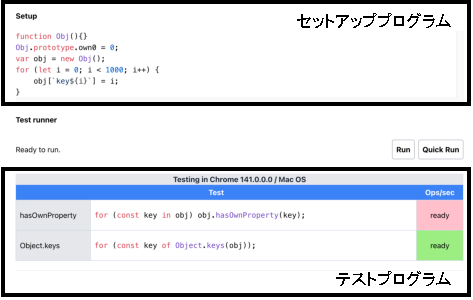
\includegraphics[width=1.0\linewidth]{./Noguchi_fig/jsPerf_example.pdf}
    \caption{マイクロベンチマーク共有サービスの投稿例\protect\footnotemark}
    \label{fig:jsPerf}
\end{figure}

\footnotetext{\url{https://jsperf.app/qiwudo}}
%----------------------

% マイクロベンチマーク共有サービスの一つであるJsPerfにおいて,実際に投稿されているマイクロベンチマークの例を図\todo{スクショ挿入・リンクをフットノート}に示す,マイクロベンチマーク共有サービスでは,1つの検証における準備を行うセットアッププログラムと,検証対象となる2つ以上のテストプログラムから構成されている.図上部に示すプログラムがセットアッププログラムを示しており,検証対象のプログラムで利用される変数の初期化などが行われている.図下部に示すプログラムがテストプログラムを示しており,図では,\todo{コードの説明}と\todo{同じく}の実行速度が計測・比較検証される.

% マイクロベンチマーク共有サービスでは,図に示すような実装対が保存・公開されており,同一の機能を異なる方法で実装した非常に短いコードの対によって構成されており,データ構造や制御構文,使用するメソッドの選択などに多様性が見られる.


%2.2
\subsection{関連研究}

Selakovicら\cite{jsRefac}は,JavaScriptを利用しているプロジェクトにおいて,開発者が高速化のために行ったリファクタリングを調査している.調査の結果,開発者は10行程度の小さい範囲の修正によって高速化への対処を行なっていることを明らかにした.この結果は,マイクロベンチマーク共有サービスで頻繁に比較される短いソースコード片の修正が,ソフトウェア高速化につながっていることを示し,本研究の動機づけとなっている.また,\cite{jsRefac}は,JavaScriptプロジェクトの解析によって10件の頻出する高速化改良パターンを作成している.この改良パターンを用いた自動修正は一定の高速化効果を示しているが,該当箇所の特定における制約などから,広範な適用には至っていない.

Turcotte ら\cite{DrAsync}は,JavaScript 言語における非同期処理に注目した性能アンチパターンを定義し,静的解析エンジンであるCodeQL\cite{ql}を利用したアンチパターンの検出と,動的解析を利用したパフォーマンスの監視を組み合わせ,修正可能な性能アンチパターンの検出を行った.本研究の静的解析による低速コードパターンの検出はこれに着想を得ている.

大森ら\cite{omori}は,マイクロベンチマーク共有サービスで公開される,実行速度が向上するプログラムを収集し,これをデータセットとして大規模な言語学習モデルをファインチューニングすることで,実行を高速化するプログラムに自動リファクタリングするモデルを作成した.この結果,マイクロベンチマーク共有サービス上のプログラムに対しては,マイクロベンチマークにおける高速な実装方法との完全一致において,ChatGPT-4oより約3倍の件数の高速化リファクタリングに成功している.しかし,適用対象がマイクロベンチマーク共有サービス上のプログラムに留まっており,\cite{jsRefac}と同様,広範な適用には至っていない.

% 本研究では,繰り返し処理に注目し,マイクロベンチマーク共有サービスで公開される実装対における低速コードから,構造的差分に基づいて低速コードパターンを抽出し,静的解析を用いた性能ボトルネックの早期検出を行うとともに,適用範囲を拡張する上での検出精度の指標について議論する.\memo{精度を上げることではなく,類似度がどのように反映されるかを見るという立場で話すような表現にしたい}

本研究では,マイクロベンチマーク共有サービスで公開される実装対における低速コードから,構造的差分に基づいて低速コードパターンを抽出し,静的解析を用いた性能ボトルネックの早期検出を行うことを目指す.本論文は,その第一歩として,繰り返し処理にターゲットを絞り,ベンチマークのソースコード片に基づき,修正することで実行速度の向上が期待されるソースコード片の検出を目的とする.



%%%%%%%%%%%%%%%%%%%%%%%%%%%
%3
\section{事前分析}
\label{sec:pre-analysis}
%%%%%%%%%%%%%%%%%%%%%%%%%%%


本研究では,大森ら\cite{omori}が作成したデータセットを分析対象とする.当該データセットは,マイクロベンチマーク共有サービスJsPerfで評価されたベンチマークの中で,実行速度に有意差があり,外的振る舞いが等しいことが検証された実装対29,809件を含む.以降,分析対象とするベンチマークで比較されたソースコード片の対をマイクロベンチマーク実装対,各実装対において,実行速度が遅いコードを低速コード,実行時間が速いコードを高速コードとする.

%3.1
\subsection{繰り返し処理を含むマイクロベンチマーク実装対}
\label{section3.1}

% \todo{図1で示すように} 繰り返し処理を含む実装対が全体の約43%(12,948対)存在する.

マイクロベンチマーク実装対を目視調査した結果,実装対の両方もしくは片方に繰り返し処理を含むものが多く存在することを確認した.特に,巨大な配列や長大な繰り返し処理を用いることで性能差が顕著になる実装対や,\texttt{for}と\texttt{for-of}のように,繰り返し処理の実装方法の違いによって実行時間に差が生じる実装対など,繰り返し処理に関する複数の特徴を確認した.
このような観察結果から,本研究ではマイクロベンチマーク実装対に対して繰り返し処理構造に着目した特徴分析を行う.対象とする繰り返し処理は,JavaScriptにおける \texttt{for},\texttt{for-of},\texttt{for-in},\texttt{while},および \texttt{do-while}の構文を対象とする.
以後,マイクロベンチマーク実装対のもつ特徴について,実施した分析内容とともに例を示す.

マイクロベンチマーク実装対の特徴分析には,各実装対のソースコードをGumTree\cite{gumtree}により抽象構文木へと変換し,実装対の抽象構文木間の差分解析を行った.差分解析の結果に対して,次の2点を確認し,繰り返し処理に関連する差分要素として収集する.\\
\noindent(1) 差分が直接繰り返し処理構造を含むか\\
\noindent(2) 差分要素の構造的な親要素に繰り返し処理を含むか\\
抽出された箇所に応じて目視で確認を行い,実装対の構造的特徴および性能差との関係を整理した.
分析の結果,マイクロベンチマーク実装対には実行速度に差が生じる繰り返し処理の使用パターンを複数確認した.具体例として,Listing~\ref{diff-loop},Listing~\ref{diff-inloop},Listing~\ref{diff-method}に,特徴となる部分について示す.

Listing~\ref{diff-loop}は,それぞれ\texttt{for-in}文を用いて配列に含まれる要素にアクセスする実装と,同様の処理を\texttt{for}文で実装したソースコード片である.ここで示すパターンは実行時間の差が,繰り返し処理の実装方法の違いに起因するパターンである.
%----------------------------------
\begin{lstlisting}[caption=Pairs with loop differences, label=diff-loop, captionpos=t, columns=flexible]
// slow
for (key in VAR_1) {
    if (!VAR_1.hasOwnProperty(key)) continue;
    VAR_2 = VAR_1[key];
}

// fast
for (var VAR_8=0; VAR_8<VAR_1.length; ++VAR_8) {
    VAR_2 = VAR_1[VAR_8];
}
\end{lstlisting}
%----------------------------------

Listing~\ref{diff-inloop}は,それぞれ\texttt{for}文内で \texttt{concat}メソッド,\texttt{push}メソッドを用いている実装対である.これは,繰り返し処理の実装方法は一致しているが,繰り返し内部で実行する処理が異なるパターンである.
%----------------------------------
\begin{lstlisting}[caption=Pairs with differences within the loop, label=diff-inloop, captionpos=t, columns=flexible]
// slow
for (var VAR_2=0; VAR_2<5000; VAR_2++)
    VAR_1 = VAR_1.concat([\"1\", \"2\"]);

// fast
for (var VAR_2=0; VAR_2<5000; VAR_2++)
    VAR_1.push(\"1\", \"2\");
\end{lstlisting}
%----------------------------------

Listing~\ref{diff-method}は,繰り返し処理を\texttt{forEach}メソッドで実装したものと\texttt{for-of}文で実装したものである.これは,メソッドによる処理とそれに代替する繰り返し処理について比較したパターンである.
%----------------------------------
\begin{lstlisting}[caption=Pairs of Method and alternative loop, label=diff-method, captionpos=t, columns=flexible]
// slow
var VAR_5 = new Set(VAR_2);
VAR_5.forEach(VAR_6 => {});

// fast
for (let VAR_7 of VAR_2) {}
\end{lstlisting}
%----------------------------------

これらの結果から,マイクロベンチマーク実装対には繰り返し処理の実装および繰り返し内部の操作内容の違いが性能差の要因の1つとして存在することが確認された.本研究では,このような繰り返し処理に関する構造の差分に基づいて低速コードの特徴を捉え,次章で述べる低速コードパターンの抽出および静的検出に利用する.


%%%%%%%%%%%%%%%%%%%%%%%%%%%
%4
\section{CodeQLクエリを用いた低速コードパターン検出手法}
\label{sec:approach}
%%%%%%%%%%%%%%%%%%%%%%%%%%%

%----------------------
\begin{figure*}[t]
    \centering
    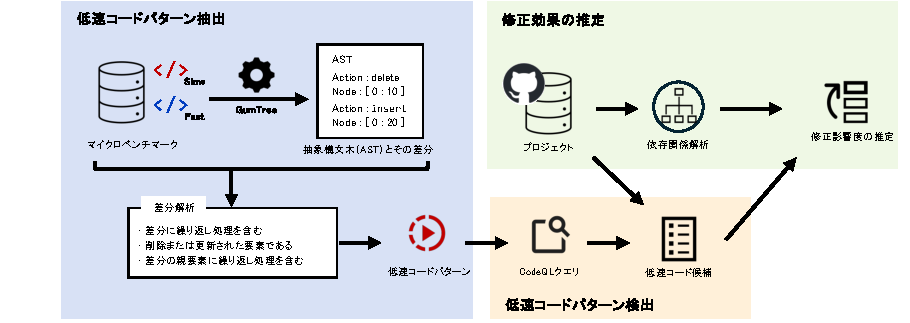
\includegraphics[width=0.9\linewidth]{./Noguchi_fig/approach_abst.pdf}
    \caption{本研究の概略図}
    \label{fig:Approach}
\end{figure*}
%----------------------

本研究では,実行速度の向上が期待されるソースコード片の検出に向けて,
マイクロベンチマーク共有サービスで実行速度が比較されたソースコード片の構造差分から低速コードパターンを作成する.これを利用し,静的解析エンジンCodeQLを用いて,ソースコード中から低速なソースコード片の候補を検出する.図\ref{fig:Approach}は,本研究で提案する手法の概略図を示す.本章では,3つの方法で構成する手法を順に述べる.
% (1) マイクロベンチマーク実装対より,低速コードの特徴を実装対の構造的差分から抽出し,低速コードパターンを作成する.作成したパターンをもとに静的解析エンジンCodeQL\cite{ql}を用いて,ソースコード中の低速コードを静的に検出する手法を提案する.また,検出結果について,修正効果の高い箇所をプログラム中の依存関係の数から推定する.以降でその詳細を述べる.


%4.1
\subsection{分析対象ベンチマークの収集}

\ref{sec:pre-analysis}章で述べたように,著者らはマイクロベンチマーク共有サービスにおいて,繰り返し処理の構造の違い,繰り返し処理の内部の操作内容の違い,などが性能差の要因の1つであることを確認した.本研究では,従来研究\cite{omori}で対象とするベンチマークの中で,比較されるソースコード間の差分に直接繰り返し処理構造を含む,または,差分要素の構造的な親要素に繰り返し処理が含まれるベンチマーク実装対を収集する.
% \memo{数を載せるか検討} 結果として29,806件の実装対から10,760対が対象となった.


%4.2
\subsection{低速コードパターンの作成}
収集した各ベンチマーク実装対において,低速コードから高速コードへ変更することを仮定し,その構造的差分を抽出する.実装対間の差分抽出には,\ref{sec:pre-analysis}章同様,GumTreeを使用し,差分要素に加え,変更操作も取得する.

次に,GumTreeによって得られた構造的差分および変更操作のうち,低速コードから削除または更新された要素を抽出する.これらの要素は,高速コードに存在しない要素であり,低速コード特有の処理や構造を示す要素であると考えられるため,低速コードの特徴候補として収集する.Listing~\ref{diff-loop}に示す実装対にこの処理を行うと,Listing~\ref{candidates}における,背景色のついた要素が低速コードの特徴候補として収集できる.

次に,収集した低速コードの特徴候補の中から,繰り返し処理およびその条件,メソッド呼び出し,配列・オブジェクト操作を,低速コード特有の実装方法を表現する有効な要素として抽出する.最後に,抽出した要素を低速コード内の開始位置,終了位置および,階層情報に基づいて統合する.この処理によって,マイクロベンチマークにおける複数の実装対に共通して出現する,低速コード特有の実装方法および構文的特徴を捉えた低速コードパターンを形成する.

図\ref{fig:slow_pattern}は,Listing~\ref{diff-loop}から作成した低速コードパターンを示し,当該パターンは,\texttt{if}文内で\texttt{.hasOwnProperty()}を呼び出す\texttt{for-in}文という特徴を有することが読み取れる.

%----------------------------------
\begin{lstlisting}[caption=Characteristic Candidates for Slow Code, label=candidates, captionpos=t, columns=flexible, literate=
    {for}{{\textcolor{black}{\colorbox{lightred}{for}}}}{3}
    {key}{{\textcolor{black}{\colorbox{lightred}{key}}}}{3}
    {in }{{\textcolor{black}{\colorbox{lightred}{in}}\kern0.5em}}{3}
    {VAR\_1}{{\textcolor{black}{\colorbox{lightred}{VAR\_1}}}}{5}
    {if}{{\textcolor{black}{\colorbox{lightred}{if}}}}{2}
    {!}{{\textcolor{black}{\colorbox{lightred}{!}}}}{1}
    {hasOwnProperty}{{\textcolor{black}{\colorbox{lightred}{hasOwnProperty}}}}{15}
    {continue}{{\textcolor{black}{\colorbox{lightred}{continue}}}}{8}
    {VAR\_1\_}{{\textcolor{black}{VAR\_1}}}{6}
]
for (key in VAR_1) {
  if(! VAR_1.hasOwnProperty(key))continue;
  VAR_2 = VAR_1_[key];
}
\end{lstlisting}
%----------------------------------

%----------------------
\begin{figure}[!h]
    \centering
    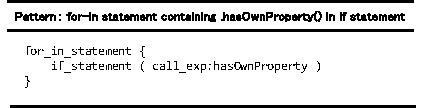
\includegraphics[width=1.0\linewidth]{./Noguchi_fig/slow_pattern.pdf}
    \caption{低速コードパターン例}
    \label{fig:slow_pattern}
\end{figure}
%----------------------



%4.3
\subsection{低速コードパターンの検出}

本研究では,低速コードパターンに基づいて検索クエリを作成し,静的解析ツールCodeQL\cite{ql}を用いて低速なソースコード片を検出する.CodeQLは,GitHubが主にセキュリティ検査を自動化する目的で開発したコード分析ツールである.具体的には,分析対象とするプログラムから抽象構文木,データフロー情報,型情報,呼び出し関係などをデータベースに保持する.このデータベースに対して,SQLに似たクエリ言語を用いて,特定の構造や振る舞いを持つソースコード検索を実現している.
本研究では,低速コードパターンをもとにCodeQLに対応するクエリに手動で変換し,ソースコード内で同様の構造を持つ箇所を検出する.


%%%%%%%%%%%%%%%%%%%%%%%%%%%
%5
\section{評価方法}
\label{sec:evaluation}
%%%%%%%%%%%%%%%%%%%%%%%%%%%

本研究では,提案手法の有効性を検証するために,作成した低速コードパターンを用いたソースコードの検出結果(低速なソースコード片の候補)を調査する.具体的には,検出結果に対し,パターン作成に使用する低速コード群との類似度を算出するとともに,検出結果を目視調査することで,低速コードパターンおよび検出結果を評価する.

低速コード群と検出した低速なソースコード片の候補との類似度は,Code2Vec\cite{code2vec}を用いてソースコード片を分散表現によりベクトル化し,コサイン類似度を用いて算出する.なお,Code2Vecは,\cite{saiki}より,JavaScriptに対応したパスコンテキスト変換処理と学習モデルを利用する.

% パターンの元となった低速コードと類似度の高いソースコード片上位\todo{n}件とを選択し,低速コードパターンの元となった実装対との類似度を算出する.次に,目視により各検出箇所が,クエリの元となったマイクロベンチマーク実装対における低速コードの特徴を正しく捉えているかを確認する.
% 各類似度指標と目視確認結果と照らし合わせることで,どの指標・閾値設定が低速コード検出に最も有効であるかを議論する.

%%%%%%%%%%%%%%%%%%%%%%%%%%%
%6
\section{ケーススタディ}
\label{sec:case-study}
%%%%%%%%%%%%%%%%%%%%%%%%%%%

\subsection{低速コードパターンとCodeQLクエリの作成}

本研究では,繰り返し処理を含むマイクロベンチマークから,6件の低速コードパターンを作成した.表\ref{tab:slow_code_patterns}は,作成した6パターンと,各パターンの作成に使用したベンチマーク数(元実装対数)を示す.これら6パターンをもとにCodeQLで実行するクエリを作成し,その妥当性を検証するために,全29,809件のベンチマーク実装対を対象として検出数を調査した.結果は表中の「検索結果」として示す.検索結果には,各パターンの作成に使用したベンチマークが含まれたため,再現率は100\%となり,作成したクエリが妥当であることが確認できた.ただし,マイクロベンチマーク実装対には,対象となるパターンを含んでいたとしても,そのパターンの実行時間を比較することを目的としないものも多く含まれるため,適合率は6.9\%~47.4\%に留まった.したがって,GitHub上のリポジトリを対象に同様の検索を行った場合にも,対象となる低速コードパターンに対して,偽陽性となるソースコード片が一定数検出される可能性が示唆される.

%----------------------¬
\begin{table}[t]
    \centering
    \caption{低速コードパターン}
    \label{tab:slow_code_patterns}
    \setcounter{patternID}{0} % 表が始まる前にカウンタを0にリセット
    \resizebox{1.0\linewidth}{!}{
        \begin{threeparttable}
            \begin{tabular}{clrr}
                \toprule
                \textbf{ID} & \textbf{特徴} & \textbf{元実装対数\tnote{*}} & \textbf{検索結果} \\
                \midrule
                
                \refstepcounter{patternID}\label{ptn:for-in}
                \thepatternID & for-in文 & 351 & 1042 \\
                
                \refstepcounter{patternID}\label{ptn:forEach}
                \thepatternID & .forEach()呼び出し & 328 & 692 \\
                
                \refstepcounter{patternID}\label{ptn:hasOwnProperty}
                \thepatternID & if文に.hasOwnProperty()呼び出しを持つfor-in文 & 78 & 201 \\
                
                \refstepcounter{patternID}\label{ptn:json}
                \thepatternID & .parse(.stringify())呼び出し & 27 & 72 \\
                
                \refstepcounter{patternID}\label{ptn:applymap}
                \thepatternID & .apply().map()呼び出し & 11 & 188 \\
                
                \refstepcounter{patternID}\label{ptn:push}
                \thepatternID & .push()呼び出しを持つfor-of文 & 10 & 28\\
                \bottomrule
            \end{tabular}
            
            \begin{tablenotes}
                \raggedleft
                \item[*] 各パターンの作成に使用したベンチマーク実装対の数
            \end{tablenotes}
        \end{threeparttable}
    }
\end{table}
%----------------------

%6.2
\subsection{低速コードパターンの検出}

ケーススタディとして,本研究では,分散バージョン管理システムGitHubで公開されているリポジトリを対象に低速コードパターンの検出を行う.対象とするリポジトリは,主要言語がJavaScript,最終コミットが1年以内のプロジェクト,スター数上位1,000プロジェクトを選定し,2025年10月13日時点で最新のスナップショットを分析対象とした.

表\ref{tab:result_detect}は,表\ref{tab:slow_code_patterns}に示した各低速コードパターンの検出結果を示す.表中には,パターンID,1つ以上のソースコード片が検出されたリポジトリ数,単一リポジトリにおける最大検出数,1,000プロジェクトにおける総検出数を示す.

表\ref{tab:result_detect}から,パターン間で検出数に違いはあるものの,各低速コードパターンは,48プロジェクトから842プロジェクトで検出された.表\ref{tab:slow_code_patterns}におけるID\ref{ptn:for-in}や,ID\ref{ptn:forEach}の低速コードパターンのように,マイクロベンチマーク実装対における該当数が多いパターンは実プロジェクトにおいても検出数が多かった.なお,これらのパターンは一般的に利用される繰り返し処理の構文であることから,検出数が多いことは妥当である.\todo{もう一言,結果を述べたい!}\todo{パターン2はforeachだから多いのは予想通り?パターン5が少ないのは最近のJSではapplyを使わずにスプレッド構文を使うことが増えているから?まぁ,もともとの該当数も少ないですけどね.}\todo{パターン6は,実行速度としてはforとpushを使うほうが速いですが,for-ofのほうが可読性が高い書き方なので,ソフトウェア開発では好まれる?}
また,

%----------------------
\begin{table}[t]
    \centering
    \caption{低速コードパターンに基づく検出結果}
    \label{tab:result_detect}
    \resizebox{1.0\linewidth}{!}{
        \begin{tabular}{crrr}
            \toprule
            \textbf{ID} & \textbf{検出リポジトリ数} & \textbf{最大検出数 (件)} & \textbf{総検出数 (件)} \\
            \midrule           
            \ref{ptn:for-in} & 689 & 7,378 & 90,592 \\
            \ref{ptn:forEach} & 842 & 12,675 & 161,681 \\
            \ref{ptn:hasOwnProperty} & 308 & 1,125 & 9,516 \\
            \ref{ptn:json} & 282 & 142 & 2,684 \\
            \ref{ptn:applymap} & 48 & 12 & 138 \\
            \ref{ptn:push} & 477 & 3,351 & 30,075 \\
            \bottomrule
        \end{tabular}
    }
\end{table}
%----------------------

%----------------------
\begin{figure}[t]
    \centering
    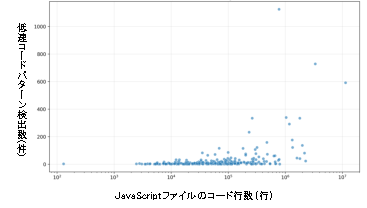
\includegraphics[width=1.0\linewidth]{./Noguchi_fig/ID3_222_log.pdf}
    \caption{低速コードパターンID3による検出数と規模\todo{縦軸も対数軸にできない?あと,縦軸名は縦書きではなく横書きで90度傾ける}\todo{横軸は対数表記なら,$10^1$, $10^2$のように書くべき}}
    \label{fig:plot_id3}
\end{figure}
%----------------------

また,図\ref{fig:plot_id3}は,ID~~\ref{ptn:hasOwnProperty}について,リポジトリ規模に対する検出数の関係を示す.横軸はリポジトリに含まれるJavaScriptファイルの総行数,縦軸は検出数を示す.プロジェクト規模が大きくなるほど低速コードパターンの検出数が増加する傾向があり,スピアマンの順位相関係数は\todo{X}となり,正の相関が認められる.他の低速コードパターンによる検出結果についても,同様の傾向が見られた.

%6.3
\subsection{検出結果の類似度}

本研究では,提案手法の有効性を検証するために,検出したソースコード片群と,パターン作成に使用する低速コード\todo{群?}との類似度を総当たりで算出した.誌面の都合上?
%Code2Vecにおける分散表現取得の計算時間の都合上,
パターンID \ref{ptn:hasOwnProperty}「if 文に.hasOwnProperty() 呼び出しを持つ for-in 文」を対象とした実験を示す.なお,長大,または文法的に不正なソースコード片は,Code2Vecによる分散表現取得における構文解析で失敗するため対象外とするため,検出総数9,516件中,分散表現の取得に成功した7,039件を用いる.


検出したソースコード片と,表\ref{tab:slow_code_patterns}に示すID \ref{ptn:hasOwnProperty}のパターン作成に使用した低速コード\todo{群?}78件を対象に,それぞれコサイン類似度の結果を箱ひげ図で示す.左側の箱ひげ図(ID3検出結果)中の点は,検出した各ソースコード片別に,ベンチマーク群と総当たりでコサイン類似度を算出した平均値の分布を示す.右側の箱ひげ図(マイクロベンチマーク)中の点は,パターン作成に使用したベンチマークに対し,それを除くベンチマークと総当たりでコサイン類似度を算出した平均値の分布を示す.なお,ID \ref{ptn:hasOwnProperty}における低速コードパターンを持つ低速コードの例は,Listing~\ref{diff-loop}に示す.


% 次に,本手法によって検出されたソースコード片について,Code2Vecを用いて分散表現を取得し,低速コードパターンの元となった低速コードとコサイン類似度を計算する.Code2Vecにおける分散表現取得の計算時間の都合上,対象パターンをID \ref{ptn:hasOwnProperty}「if 文に.hasOwnProperty() 呼び出しを持つ for-in 文」に限定する.なお,長大,または文法的に不正なソースコード片は,Code2Vecによる分散表現取得における構文解析で失敗するため,検出総数9,516件中,分散表現の取得に成功した7,039件を用いる.
% 検出したソースコード片と,表\ref{tab:slow_code_patterns}に示す,ID \ref{ptn:hasOwnProperty}の低速コードパターンを持つ低速コード78件について,それぞれコサイン類似度を算出し,その平均値について図\ref{fig:boxplot_cosine}に示す.なお,ID \ref{ptn:hasOwnProperty}における低速コードパターンを持つ低速コードの例は,Listing\ref{diff-loop}に示している.

% 比較対象として,マイクロベンチマーク実装対の低速コードに対し,CodeQLを用いた低速コードパターン検出を行い,検出したソースコード片123件について,同様にコサイン類似度を計算した結果を図\ref{fig:boxplot_cosine}の右側に示す.

%----------------------
\begin{figure}[t]
    \centering
    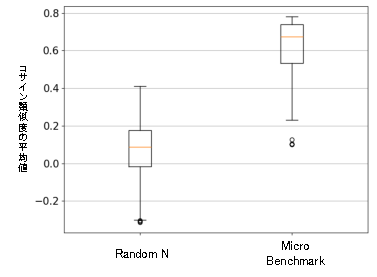
\includegraphics[width=1.0\linewidth]{./Noguchi_fig/boxplot_compare.pdf}
    \caption{低速コードパターンID \ref{ptn:hasOwnProperty}で検出されたソースコード片とパターン元低速コードのコサイン類似度}
    \label{fig:boxplot_cosine}
\end{figure}
%----------------------

ID3検出結果の平均値は0.08,中央値は0.09である一方,マイクロベンチマークでは,平均値は0.61,中央値は0.68となった.コサイン類似度の高い検出例について,実プロジェクトにおけるソースコード片と,マイクロベンチマーク実装対におけるソースコード片をそれぞれ,Listing\ref{ID3_highcos}とListing\ref{MB_highcos}に示す.
Listing\ref{ID3_highcos}におけるコサイン類似度の平均値は0.39であり,Listing\ref{MB_highcos}におけるコサイン類似度の平均値は0.78である.
Listing\ref{diff-loop}とListing\ref{MB_highcos}および,コサイン類似度の値に示すように,マイクロベンチマーク実装対においては,変数名などが同じ規則で抽象化されており,加えてコード長が近いことによって,様々なコード長および多様な変数名を持つ.実プロジェクトにおけるソースコード片と比べて,コサイン類似度が大きいことがわかる.なお,目視でコサイン類似度とソースコード片を確認したところ\memo{上位10・第1〜第3四分位数のそれぞれ10・下位10の計50個を目視.載せるか&目視増やすか&見る箇所変えるかは検討},目的とした低速コードパターンについては,コサイン類似度の大きさに関わらず含まれていることを確認した.

類似度が高いソースコード片が検出できた一方で,6.1節でも述べたように,繰り返し処理の性能効率性を比較することを目的としないソースコード片も検出しているため,類似度の低いソースコードが多数検出されていることが示唆される.Listing\ref{ID3_highcos}とListing\ref{MB_highcos}に示すように,類似度の高いソースコード片については,比較している低速コードと,コード長および構造が類似し,変数名が短い単純なソースコード片が多く見られた.
一方,類似度が低いソースコード片では,低速コードパターンに,別の処理が追加された,全体のコード長が大きいソースコード片や,変数名が長い,リテラルを多く含むといったソースコード片が多く見られた.これに伴い,コサイン類似度が小さいほど,検出したソースコード片の構造は低速コードと比較して複雑になっていく傾向があることを確認した.

% \memo{規模感(構文解析によるコンテキスト数)の話をどこでするか.箱ひげ図の下辺が消えるだけなので図に反映させなくてもいいけど言及はするべき?.パターン元低速コードは平均で161コンテキスト.なお,ベクトル化においてコンテキスト数は200に押し込められるため,コンテキストが多いほど情報が削ぎ落とされたベクトルになる.}




%----------------------------------
\begin{lstlisting}[caption=実プロジェクトにおける類似度の高い検出例, label=ID3_highcos, captionpos=t, columns=flexible]
for (var key in this.defaults) {
  if (!options.hasOwnProperty(key)) {
    attr[key] = this.defaults[key];
  }
}
\end{lstlisting}
%----------------------------------


%----------------------------------
\begin{lstlisting}[caption=マイクロベンチマークにおける類似度の高い検出例, label=MB_highcos, captionpos=t, columns=flexible]
VAR_1 = {
  KEY_1: 5,
  KEY_2: 13,
  KEY_3: 8,
};
var VAR_2 = [];
for (var VAR_3 in VAR_1) {
  if (VAR_1.hasOwnProperty(VAR_3)) {
    VAR_2.push(VAR_1[VAR_3]);
  }
}
\end{lstlisting}
%----------------------------------


%%%%%%%%%%%%%%%%%%%%%%%%%%%
%7
\section{考察}
\label{sec:discussion}
%%%%%%%%%%%%%%%%%%%%%%%%%%%


%7.1
\subsection{低速コードパターンに基づく検出結果の妥当性}

本研究では,提案手法により作成した低速コードパターンおよび,CodeQLを利用した検出によって,実際のソースコード中から低速コードパターンを含むソースコード片を検出した.分析の結果,プロジェクト規模が大きいほど,低速コードパターンの検出数が増加していた.開発が進み,ソフトウェアが進化する中で性能低下が引き起こされる従来研究\cite{emprical_perfomancebug}の結果を踏まえると,規模の肥大化に伴い低速コードパターンで検出されるソースコード片が増加すること驚く結果ではなく,ソフトウェア全体としてのボトルネックとなっていないのであれば,検出数が増えることが必ずしも問題とは言えない.今後の研究で,検出したソースコード片がソフトウェア全体のボトルネックとなるかを明らかにするために,検出方法を開発した.本手法は偽陽性が多い点もあるが,低速コードパターンを使った実装も検出できているため,CodeQLの利用した静的な低速コードパターンの検出方法は有効であることを示すことができた.

% 作成した6件の低速コードパターンおよび,その検出結果は妥当であると考えられる.\memo{これを主張するほどの結果とはいえない?}
% また,これに伴い,静的な低速コードパターンの検出において,CodeQLの利用が有効であることが示唆された.

% 一方で,プロジェクト中で,表\ref{tab:result_detect}の最大検出数に示すように,低速コードパターンの検出数が多い場合,全てを高速コードに変更することは現実的ではなく,修正効果の大きい箇所を選択して示すことで,より効果的な低速コードパターンの検出となることが考えられる.


%7.2
\subsection{類似度指標}

提案手法による低速コードパターンの検出結果に対して,コサイン類似度による評価と目視調査の結果から,CodeQLにより検出されたコード片は,低速コードパターンを含んでおり,作成したクエリが構造的に妥当であることを確認した.
また,検出されたソースコードに対するコサイン類似度の値について,コサイン類似度は,コード間の構造的,意味的な類似度を計測できる一方で,ソースコード片の長さや変数名など,低速コードパターンとは無関係な要素の影響も受ける.したがって,多様な変数名や処理を含む実プロジェクトの検出結果に対するコサイン類似度の値は,マイクロベンチマーク実装対の値と比較して小さくなるため,検出結果が正しいと判断できる類似度の値域について今後検討する.

なお,低速コードパターンの元となった低速コードとコサイン類似度の高いソースコード片は,マイクロベンチマーク実装対と比較し,コード長や処理内容が類似することから,マイクロベンチマークを参照した修正が比較的容易に適用できる箇所である可能性を示している.したがって,検出結果に対するコサイン類似度を用いた評価は,マイクロベンチマークを用いた性能改善の容易性を示す指標として有用である可能性が示唆される.

\memo{体感0.2ぐらいの類似度が規模感の近さと修正できそう感の閾値.0.1を下回ると目視しんどいレベルのサイズが増える}


\subsection{妥当性の脅威}

%7.3
\noindent\textbf{内的妥当性: }
本研究では,低速コードの特徴抽出をGumTreeによる差分解析に依存している.したがって,抽出された差分が必ずしも低速コードの特徴を正確に表現していない可能性が存在する.本研究では,差分から得られた要素を目視により確認し,実装例と照合した上でパターンを作成しているため,その影響は小さいと考えるが,今後パターン数を拡張する際には,差分抽出の精度や作成手法の改善が課題となる.

また,低速コードパターンの検出におけるパターンのクエリ化を,GumTreeによる差分解析結果をもとに手作業で行っている.そのため,作成したクエリが低速コードパターンを正確に反映しているかについては,目視による確認に依存しており,一定の主観的判断が含まれる.ただし,本研究では,マイクロベンチマークに対して実際にクエリを適用し,想定した低速ソースコード片が検出されることを確認しており,その影響は限定的であると考える.

本研究で利用したマイクロベンチマーク共有サービスであるJsPerfは2020年にサービスを終了しており,当時の高速実装が現在においても最適であるとは限らない.この点については,関連研究\cite{omori}においても同様の指摘がなされている.

本研究における類似度計測においては,プログラム断片のベクトル化にCode2Vecを利用している.Code2VecはJavaおよびC\#を対象としているため,それらの言語への利用における精度と差異が生じる可能性がある.本研究ではJavaScript対応かつマイクロベンチマークをもとに学習された学習モデル\cite{saiki}を使用することで,この影響を抑えるよう努めた.
なお,分散表現の取得における内部処理において,学習の設定に応じて,ソースコード片のトークン数や抽象構文木における構造における制限や,分散表現化に利用する特徴のフィルタリングが発生するため,コード長の大きいソースコード片については,分散表現において,十分にその特徴を反映できていない可能性がある.変数名の抽象化や,学習モデルの再構築によって改善が期待されるものの,開発初期における性能ボトルネックの検出が本研究の目的であることから,本研究において,長大なコードへの対応に関する影響は小さいと考える.

\noindent\textbf{外的妥当性: }
本研究におけるケーススタディでは,時間的制約のため,GitHub上のスター数上位のプロジェクトに対象を限定して分析を行った.そのため,結果の一般性は限定的である可能性がある.
特にスター数の多いプロジェクトは,既に十分に最適化・保守が行われていることが多いため,このようなプロジェクトにおける検出結果は,一般的な開発段階のソフトウェアとは異なる可能性がある.

また,本研究では,低速コードパターンを6個作成し,ケーススタディを実施した.また,類似度計測ではそのうち1つのパターンについての検証となっている.異なるパターンに対しては,同様の手法で実験を行う必要があり,複数パターンに基づく評価によって,提案手法の汎用性および有効性をさらに検証することが今後の課題である.


%%%%%%%%%%%%%%%%%%%%%%%%%%%
%7
\section{おわりに}
\label{sec:summary}
%%%%%%%%%%%%%%%%%%%%%%%%%%%

本研究では,ソフトウェア中に潜在する,修正によって実行速度の向上が期待されるソースコード片を検出することを目的とし,繰り返し処理にターゲットを絞り,マイクロベンチマーク共有サービスで提供されるベンチマーク実装対の構造差分から低速コードパターンを抽出し,静的解析エンジンであるCodeQLを用いて実際のソースコード中から低速コードを検出する手法を提案した.

ケーススタディとして,6件の低速コードパターンおよび,それぞれに対応するCodeQLクエリを作成し,GitHub上の実プロジェクト1,000件を対象に検出実験を行った.その結果,提案手法によって作成した低速コードパターンが実際のソースコード中から検出され,マイクロベンチマーク共有サービス由来の構造差分が,実際のプログラムにおける処理構造を適切に捉えていること,および,低速コードパターンの検出において,CodeQLによる静的検出が有効であることを確認した.

さらに,提案手法によって検出されたソースコード片に対して,Code2Vecを用いて分散表現を取得し,コサイン類似度による評価および目視調査を実施した.その結果,CodeQLによって検出されたコード片はいずれも低速コードパターンを含んでおり,作成したクエリが妥当であることを確認した.一方で,コサイン類似度は構文的な類似性に加え,コードの長さや変数名などの表層的な特徴に影響される傾向が見られた.したがって,実プロジェクトにおいて検出された,コサイン類似度の高いソースコード片は,マイクロベンチマークのソースコードとコード長や処理構造が類似するため,マイクロベンチマークを用いた性能改善の容易性を示す指標として有用である可能性が示唆された.

今後の課題として,繰り返し処理に限らず,低速コードパターン作成における差分抽出や低速コードの特徴量抽出の手法,およびクエリ作成方法の拡張を進めることが挙げられる.また,検出結果に対して,コサイン類似度や,その他の評価指標の検討を通じて,より意味的な類似性を捉えられる指標の構築を目指す.
これらを元に.高速化修正の可否および,修正の効果,影響範囲の推定を行うことで,より効果的な性能ボトルネック検出および修正候補の提示手法の構築を目指す.

\begin{acknowledgment}
本研究はJSPS科研費 25K15058の助成を受けたものである.
\end{acknowledgment}



\bibliographystyle{ipsjunsrt}
\bibliography{bibnoguchi}

\end{document}
